



Collecting human brain measurements is not easy to task since the the tissues has to be extracted not long after the subject death. So while each can be represented in more details and much cheaper to extract as time goes by, the number of samples is still extremely limited. This is even more acute when we compare the number of available samples (few dosen) to the dimention of representation (in the tens of thousands).
Unfortunately, there is no dataset that measure single cell profiles in the human brain. This posses a great challenge but also a great opportunity for blind-demixing. 
We use the brainspan dataset \cite{brainspan} to 
NMF since it is clear that using single cell profiles the profiles


We used brainspan data from {\bf{K}} different region which was gathered from 8 humans subjects (we limit our analysis only to adult humans older than 17). There are ~8 samples from each region. Each expression is represented by a vector of 52376 which hold sequencing data both for coding region in the DNA and for non-coding regions. 

To evaluate the data we computed correlation between the reconstructed profiles and single cell profiles that were gathered in the mouse \cite{barres2014}. We mapped the genes in the human to their orthologs in mouse and computed the spearman correlation between the reconstructed profiles and each of the single cell profiles.

We compared our results with those of random baseline that was obtained by selecting a set of 3 sample as the reconstructed profiles. Our reconstructed profiles are well above the baseline. It should be notated that even single cell experiments that are gathered from the same species in different experiment and from different region is only correlated to the other samples from the same type by 0.8XXX. 

We find that in our reconstructed profiles the gene that are
The ordering of the genes in the reconstructed profiles is enriched by...





\begin{figure}[!hbt]
   (a) \hspace{120pt}(b) \hspace{120pt}(c) \hspace{120pt}
   \centering
     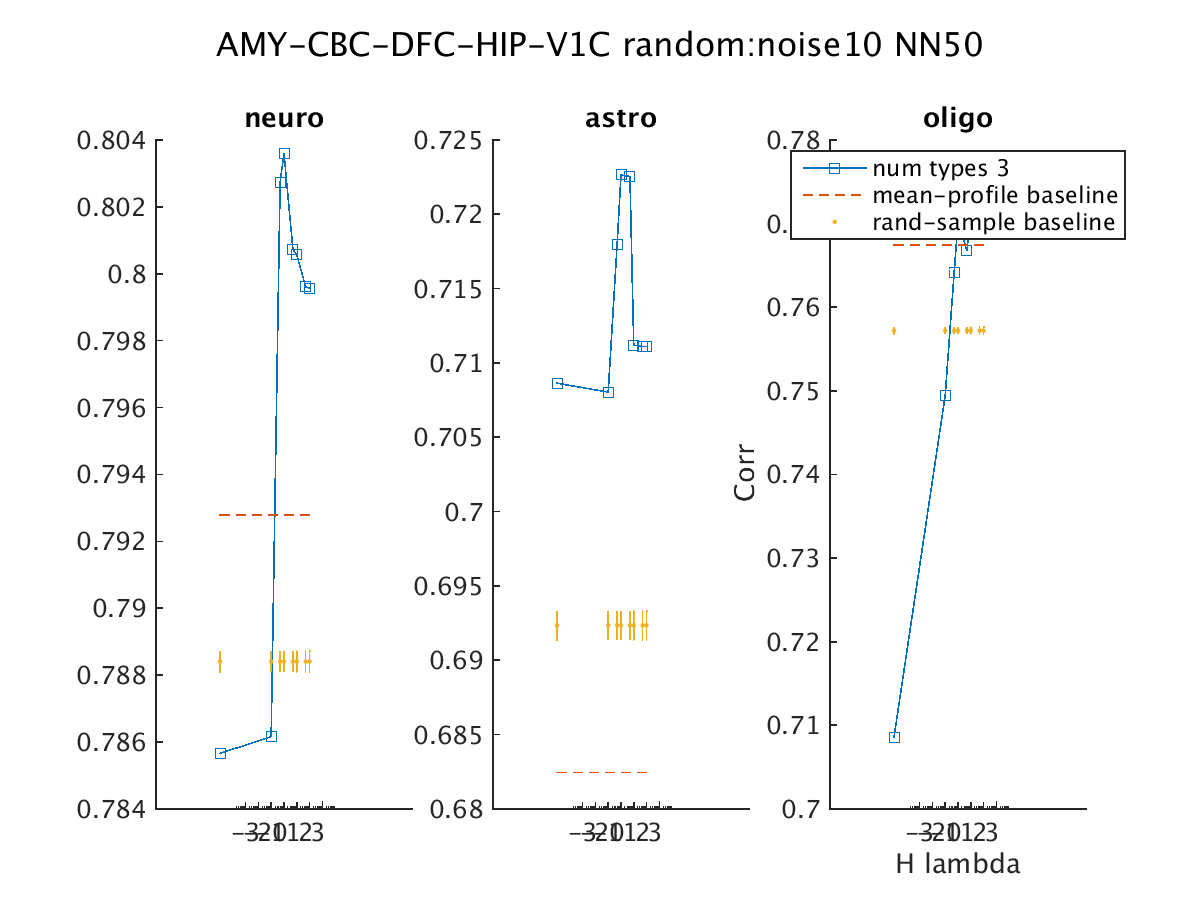
\includegraphics[width=0.95\textwidth]{human_data}
     caption{The effect of $\lambda$ on reconstruction}, 
    (a)  With a single region, all optimization method perform better as we introduced more samples. With a limited number of samples the active set and the block pivoting approaches performed the best. (b) Using multiple regions, the regularized connection between the region profiles help to reconstruct the original profiles. This is especially noticeable when only few samples are available for each region. (c) ????
    \label{fig:controlled_exp}
\end{figure}
